\section{Aufbau der Spielarchitektur}

\subsection{Überblick}

Slick2D stellt Techniken zur Umsetzung eines zustandsbasierten Spieles zur Verfügung.
In Abbildung \ref{fig:spielarchitektur:states} werden die Zustände des Spiels und ihre Reihenfolge gezeigt.

Ein Spiel startet im \texttt{MainMenuState}.
Hier kann der Spieler das Spiel entweder direkt beenden oder in den \textit{LevelMenuState} wechseln.
Der \texttt{LevelMenuState} bietet eine Auswahl aller zur Verfügung stehenden Levels an, welche dann im \texttt{PlayingState} gespielt werden können.
Während des Spiels kann das Spiel durch Wechsel in den \texttt{PauseMenuState} pausiert werden.
Nach erfolgreichem oder nicht erfolgreichem Abschluss eines Levels bietet der \texttt{GameFinishState} die Möglichkeit das Level zu wechseln, das Level erneut zu spielen oder das Spiel zu beenden.

\begin{figure}[]
\centering
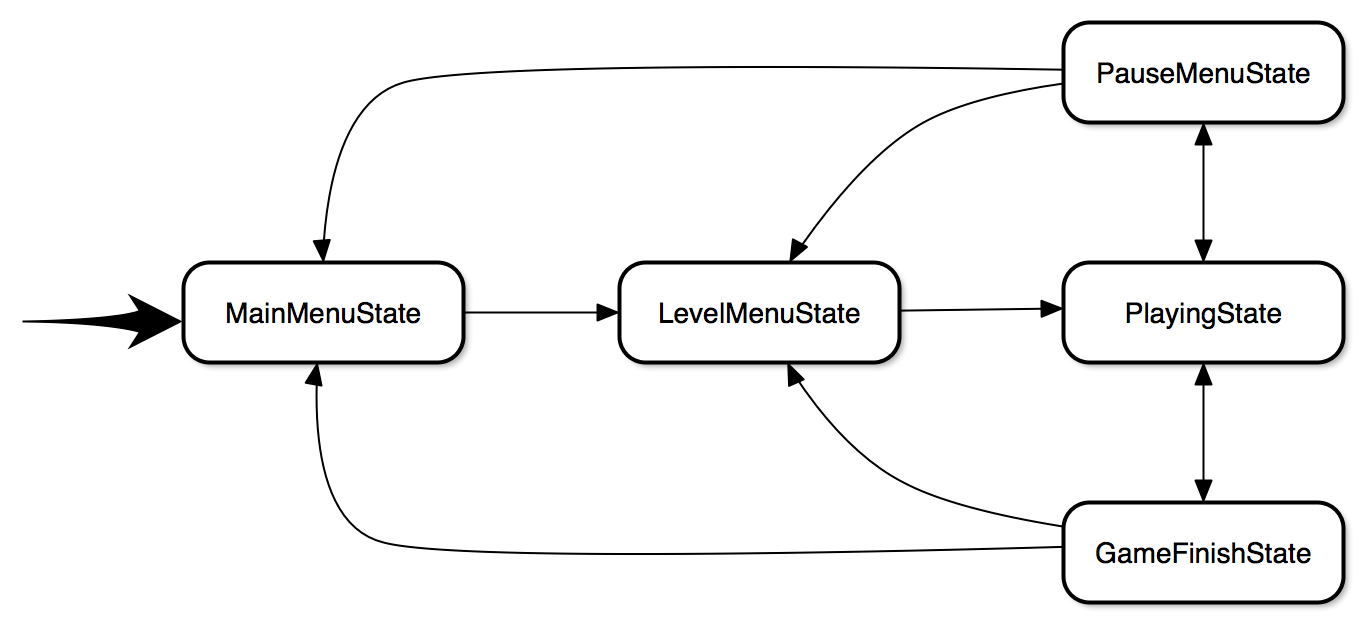
\includegraphics[width=3in]{img/05_states.png}
\caption{Übersicht der Zustände des Spiels}
\label{fig:spielarchitektur:states}
\end{figure}

Im FMC-Diagramm in Abbildung \ref{fig:spielarchitektur:fmc} wird die Bedeutung des \texttt{PlayingState} sowie der Aufbau eines Levels deutlich.
Der \texttt{PlayingState} empfängt die Eingaben des Spielers und reicht diese an den \texttt{LevelController} weiter.
Der \texttt{LevelController} kontrolliert und steuert die Bestandteile eines Levels.

\begin{figure}[]
\centering
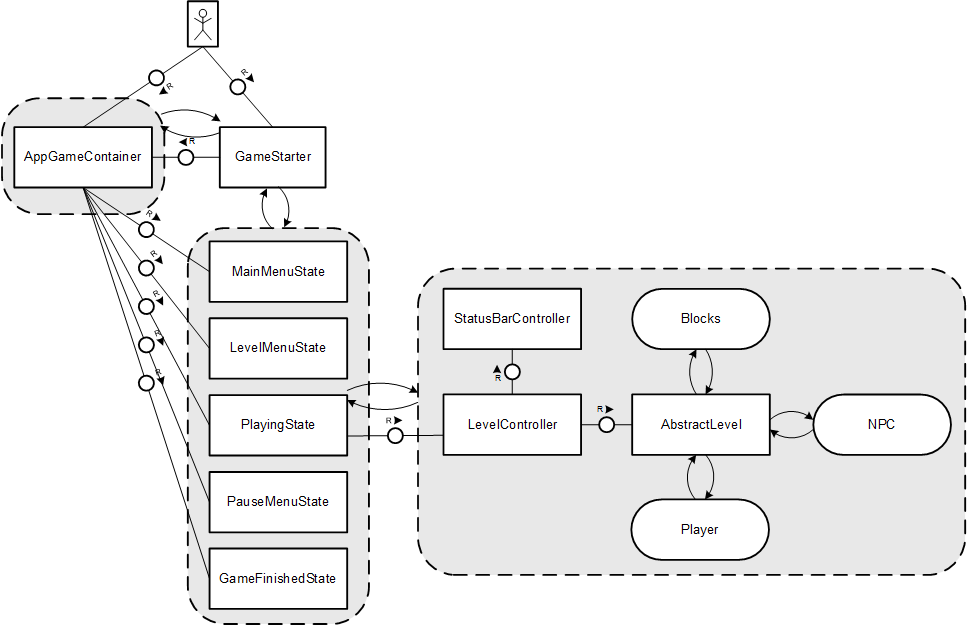
\includegraphics[width=3in]{img/05_fmc.png}
\caption{FMC Diagramm des Spiels}
\label{fig:spielarchitektur:fmc}
\end{figure}

\subsection{Level}

Jedes Level erbt von \texttt{AbstractLevel}.
In Abbildung \ref{fig:spielarchitektur:abstractlevel} wird der Aufbau eines Levels deutlich.
Ein Level besteht aus einer Menge an \texttt{NPC}-Objekten, welche die Gegner repräsentieren.
Außerdem beinhaltet es ein \texttt{Player}-Objekt sowie die Menge der Blöcke(\texttt{Block}), also der Karte des Levels.
Eine Übersicht über alle verwendbaren Spielobjekte wird in Abbildung \ref{fig:spielarchitektur:model} gegeben.
Level sind komplexe Datentypen und verstehen sich als Komposition der, in Abbildung \ref{fig:spielarchitektur:model} gezeigten, spielspezifischen \texttt{GameObject} Datentypen.
Zur Vermeidung von Redundanz und zur klaren Trennung zwischen Modell und Controller wird die Steuerung der Elemente eines Levels durch den \texttt{LevelController} übernommen.
Durch diese Trennung eignen sich Implementierungen von \texttt{AbstractLevel} sehr gut zur Erzeugung durch eine anwendungsspezifische Sprache.

\begin{figure}[]
\centering
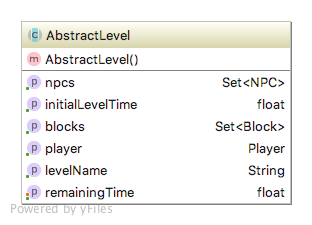
\includegraphics[width=2in]{img/05_abstractlevel_uml.png}
\caption{UML Darstellung der Klasse AbstractLevel}
\label{fig:spielarchitektur:abstractlevel}
\end{figure}

\begin{figure}[]
\centering
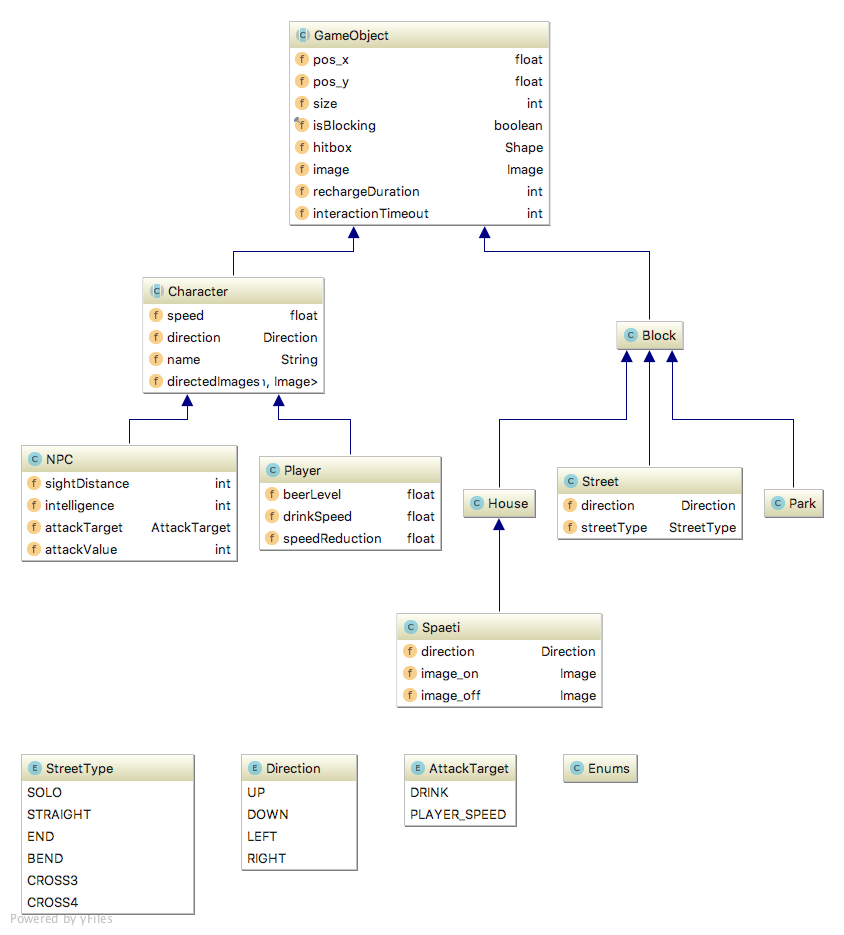
\includegraphics[width=3in]{img/05_model.png}
\caption{Spielobjekte}
\label{fig:spielarchitektur:model}
\end{figure}

\subsection{LevelController}

- Initialisiert ein Level zur Benutzung (Blockpositionen ...)
- Erhält die Eingaben des Nutzers und wandelt diese in Änderungen des Levels um
- steuert die KI
\todo{stubs}

\subsection{Highlights der Implementierung}

Ideen:
- LevelMenu
- Kollisionskontrolle
- KI